%%%%%%%%%%%%%%%%%%%%%%%%%%%%%%%%%%%%%%%%%%%%%%%%%%%%%%%%%%%%%%%%%%%%%%
\section{Basic Design}\label{sec:design}
%%%%%%%%%%%%%%%%%%%%%%%%%%%%%%%%%%%%%%%%%%%%%%%%%%%%%%%%%%%%%%%%%%%%%%

% Basic idea
%In this section we describe the design and implementation of %Casper.
PMPI is the name shifted profiling interface to support profiling
and tracing tools of MPI \cite{mpi30-report}. Casper is designed
as an external library through the PMPI interface so that it is able
to transparently link with various MPI implementations, by
overloading necessary MPI functions and leveraging wrappers to them.
Casper deploys background ghost processes in each node to assist
RMA operations that are from other interconnected processes and
internally require software intervention on the target side. In this
section, we present the basic design of Casper for supporting
background ghost processes.


%%%%%%%%%%%%%%%%%%%%%%%%%%%%%%%%%%%%%%%%%%%%%%%%%%%%
\subsection{Process Management}\label{sec:des-pe}
%%%%%%%%%%%%%%%%%%%%%%%%%%%%%%%%%%%%%%%%%%%%%%%%%%%%

The strategy of process management for Casper ghost processes
requires attention to two issues. First, Casper should never
leverage new processes if there is no idle core in the node;
otherwise it may cause core oversubscription and severely degrade
performance. Dedicating some cores to perform asynchronous progress
discharging others from doing so is beneficial in many scenarios as we
will demonstrate in Section~\ref{sec:eva}. Assessing the number of idle cores within the MPI stack,
however, is not trivial, and there may exist non-MPI processes as
well. Therefore, a generalized solution is to allow users to specify
the number of available ghost processes for each node through an
MPI execution argument or host files.

The second issue is that user applications should be unaware
of these background processes during their execution. However,
a ghost process is initialized as a background MPI process
internally connecting with user processes. Since the most
commonly used MPI communicator, \texttt{MPI\_COMM\_\-WORLD},
contains these processes, Casper defines a communicator called
\texttt{COMM\_\-USER\_WORLD} that contains all the regular
processes only, as shown in Figure~\ref{fig:deg-user-comm}.
\texttt{COMM\_USER\_WORLD} is exposed to user applications instead of
\texttt{MPI\_COMM\_WORLD} as a transparent replacement during the
whole execution. The following guarantees that the ghost
processes are never able to be exposed to user applications.

\begin{figure}
\centering
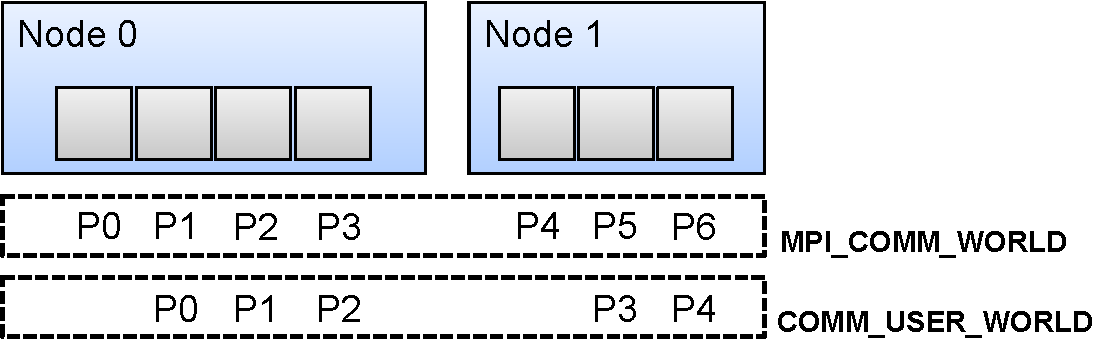
\includegraphics[width=0.9\columnwidth]{figures/casper/design_user_comm.pdf}
\caption{User world communicator.}
\label{fig:deg-user-comm}
\end{figure}

\begin{enumerate}

\item For any MPI function that is able to expose the accessibility of
  the original \texttt{MPI\_COMM\_WORLD} to user applications,
  Casper wraps it and internally exchanges the communicator with
  \texttt{COMM\_USER\_WORLD} if it is equal to
  \texttt{MPI\_COMM\_WORLD}.

\item For an MPI function that creates a new communicator, a ghost
    process will never be included in the new communicator, because
    the base communicator from which the new one is created has
    already been exchanged in the previous
    step and hence it does not contain the ghost processes.

\item An MPI function will never receive an input parameter that
    is a user-defined communicator containing ghost processes,
    because users are never able to create such communicators (as
    described in the second step).
\end{enumerate}



%%%%%%%%%%%%%%%%%%%%%%%%%%%%%%%%%%%%%%%%%%%%%%%%%%%%
\subsection{Initialization and RMA operation redirection}\label{sec:des-init}
%%%%%%%%%%%%%%%%%%%%%%%%%%%%%%%%%%%%%%%%%%%%%%%%%%%%

After MPI initialization, ghost processes
continuously poll the MPI progress engine for receiving requests from local
user processes and handling redirected RMA operations.
When the user creates a memory window by using
\texttt{MPI\_Win\_allocate}, Casper first allocates a shared-memory
region between local user processes and the ghost process by calling
the MPI-3 \texttt{MPI\_Win\_allocate\_shared} function, as depicted in
Figure~\ref{fig:deg-mem-map}.
Then internal windows are created using those shared-memory regions
within all the processes, including ghost processes, in order to allow
RMA operations to be redirected. Finally, a user window only within
all the user processes is created and returned.

\begin{figure}
\centering
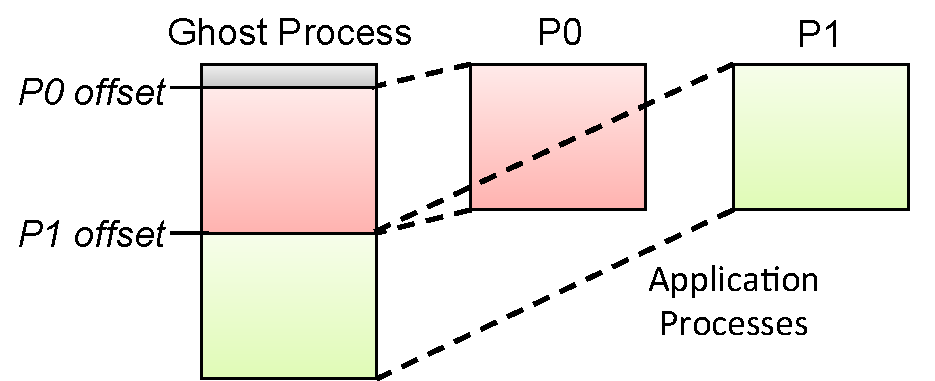
\includegraphics[width=0.9\columnwidth]{figures/casper/design_mem_map.pdf}
\caption{Casper shared buffer mapping.}
\label{fig:deg-mem-map}
\end{figure}

Once the window becomes ready, user RMA operations can be translated
to the operation issued to a corresponding ghost process. The new
target address is changed to the address of that memory location
mapped in that ghost process.